%\documentclass[11pt,aspectratio=169]{beamer}
\documentclass[11pt,aspectratio=169,handout]{beamer}

\usepackage{amsmath}
\usepackage{amsfonts}
\usepackage{amssymb}
\usepackage{graphbox}
\usepackage{sgamevar}
\usepackage{pgfplots}
\usepackage{tikz}
\usepackage{pstricks,pst-node}
\usepackage{bigdelim}
\usepackage{qrcode}
\usepackage[absolute,overlay]{textpos}
\usepackage[ruled,vlined]{algorithm2e}



% alg
\SetKwFor{Repeat}{repeat}{}{}
\SetKwComment{Comment}{$\triangleright$ }{}
\SetCommentSty{textsf}
% pgfplot settings
\usepgfplotslibrary{fillbetween}

% tikz settings
\tikzset{
    invisible/.style={text opacity=1,opacity=0},
    visible on/.style={alt=#1{}{invisible}},
    alt/.code args={<#1>#2#3}{%
      \alt<#1>{\pgfkeysalso{#2}}{\pgfkeysalso{#3}}
    },
  }
\newcommand{\nebox}[2][]{\tikz[baseline=(h.base)]\node[rounded corners,rectangle,draw,line width=0.7pt,text depth=-4.9pt,#1] (h) {#2};}
\usetikzlibrary{arrows}
% Customized colors

\definecolor{ashgrey}{rgb}{0.7, 0.75, 0.71}
\definecolor{lightblue}{RGB}{140, 201, 247}
\definecolor{darkgreen}{RGB}{113, 160, 55}
\definecolor{darkblue}{RGB}{78, 103, 200}
\definecolor{darkpurple}{RGB}{112, 48, 160}

% Hyperlink settings

\hypersetup{colorlinks,urlcolor=darkgreen}

%Beamer settings

\setbeamertemplate{navigation symbols}{} 
\setbeamertemplate{footline}[frame number]
\setbeamertemplate{itemize items}[circle]
\setbeamertemplate{section in toc}[sections numbered]
\setbeamertemplate{subsection in toc}[subsection numbered]

\setbeamercolor{section in toc}{fg=blue}

\AtBeginSection[ ]{
 \begin{frame}{Outline}
  \hypersetup{linkcolor=black}
  \tableofcontents[currentsection]
 \end{frame}
}

% Graphics settings

\graphicspath{{../Figures/}}

% PGFPlot settings

\pgfplotsset{compat = newest}

% Gamesvar settings

\setlength{\arrayrulewidth}{0.91pt}
\renewcommand{\gamestretch}{1.68}
\def\stackedpayoffs#1#2{%
 \begin{array}{c}#1\\[2mm]#2\end{array}
}

% Math

\DeclareMathOperator*{\argmax}{argmax}
\DeclareMathOperator*{\argmin}{argmin}

\newcommand\given[1][]{\:#1\vert\:}
\newtheorem{proposition}{Proposition}

% New environments

\newenvironment{itemizes}[1][1em]{
 \vspace{#1}
 \begin{itemize}
 \setlength{\itemsep}{#1}
}{
 \end{itemize}
}


% Shared title frame

\title{Game-theoretic \\ Foundations of Multi-agent Systems}

\author{Seyed Majid Zahedi}
\titlegraphic{\vspace{-4.2em} 
\includegraphics[height=5.8em]{Logos/logo2}}

\date{} 
\subject{Lecture 1} 
\logo{
\includegraphics[height=5.6em]{Logos/logo1}}
\subtitle{\vspace{2.1em}Lecture 2: Preferences and Utilities}

\begin{document}

 \begin{frame}[plain]
  \titlepage
 \end{frame}
 
 \section{Agent Preferences}
  \begin{frame}{Outcomes and Lotteries}
   \begin{itemize}[<+->]
    \item Let $O = \{o_1, \dots, o_K\}$ be set of mutually exclusive outcomes
    \item \alert{Lottery} $A$ describes a probability distribution over outcomes
    \item We write $A=\sum p_k o_k$ to indicate that $o_k \in O$ happens with probability $p_k$
    \begin{itemize}
     \item $\sum p_k = 1$
     \item E.g., $A = 0.75 o_1 + 0.25 o_2$ means $P(o_1) = 0.75$ and $P(o_2) = 0.25$
    \end{itemize}
    \item  \alert{Compound lottery} is a lottery defined based on other lotteries
    \begin{itemize}
     \item Suppose $O = \{o_1, o_2, o_3\}$
     \item Let $A = 0.2 o_1 + 0.8 o_2$ and $B = 0.4 o_2 + 0.6 o_3$
     \item $C = 0.5 A + 0.5 B$ is a compound lottery:
      $$C = 0.5(0.2 o_1  + 0.8 o_2) + 0.5(0.4 o_2 + 0.6 o_3) = 0.1 o_1 + 0.6 o_2 + 0.3 o_3$$
    \end{itemize}
   \end{itemize}
  \end{frame}

  \begin{frame}{Ordinal Preferences}
   \begin{itemize}[<+->]
    \item We define \alert{preference relation} over lotteries as follows
    \begin{itemizes}
     \item $A \succ B$ means agent strictly prefers $A$ to $B$
     \item $A \succeq B$ means agent weakly prefers $A$ to $B$
     \item $A \sim B$ means agent is indifferent between $A$ and $B$ ($A\succeq B$  and $B\succeq A$)
    \end{itemizes}    
   \end{itemize}
  \end{frame}

  \section{von Neumann–Morgenstern Rationality}
  \begin{frame}{Axioms of von Neumann–Morgenstern (VNM) Rationality}
   \begin{enumerate}[<+->]
    \setlength{\itemsep}{1em}
    \item \alert<.>{Completeness}
    \begin{itemize}[<.->]
     \item For all lotteries $A$ and $B$, either $A \succ B$ or $B \succ A$ or $A\sim B$
    \end{itemize}
    \item \alert<.>{Transitivity}
    \begin{itemize}[<.->]
     \item For all lotteries $A$, $B$, and $C$, if $A \succeq B$ and $B \succeq C$, then $A \succeq C$
    \end{itemize}
    \item \alert<.>{Independence of irrelevant alternatives}
    \begin{itemize}[<.->]
     \item For all lotteries $A$, $B$, and $C$, and $p\in [0,1]$, then $A\succeq B \Longleftrightarrow pA + (1-p)C \succeq pB + (1-p)C$
    \end{itemize}
    \item \alert<.>{Continuity}
    \begin{itemize}[<.->]
     \item For all lotteries $A$, $B$, and $C$, if $A \succeq B \succeq C$, then $ \exists p \in [0,1]$ such that $B \sim pA + (1-p)C$
    \end{itemize}
   \end{enumerate}   
  \end{frame}
  
  \begin{frame}{Auxiliary Axioms}
   \begin{Lemma}
    Given VNM axioms, for any pair of lotteries $A$ and $B$ with $A \succ B$, we have
    \begin{itemizes}[1em]
     \item<1->\alert<1>{Betweenness}: for $p\in (0,1)$, $A \succ pA + (1-p)B \succ B$
      \item<3->[] {\color{blue} Proof sketch}
     \begin{itemize}
      \item By independence, $A = pA + (1-p)A \succ pA + (1-p)B \succ pB + (1-p) B = B$
     \end{itemize}
     \item<2->\alert<2>{Monotonicity}: for any $p,q\in [0,1]$, if $p > q$, then $pA + (1-p)B \succeq qA + (1-q)B$
     \item<4->[] {\color{blue} Proof sketch}
     \begin{itemize}
      \item Define $\delta = q/p$
      \item By betweenness, $A\succ pA + (1-p)B \succ B$
      \item Apply betweenness to second part with $\delta$: $pA + (1-p)B \succ \delta[pA  + (1-p)B] + (1-\delta) B = qA + (1-q)B \succ B$
     \end{itemize}
    \end{itemizes}
   \end{Lemma}
  \end{frame}
  
 \section{von Neumann–Morgenstern Utilities}
  \begin{frame}{von Neumann-Morgenstern Utility Theorem}
   \begin{theorem}[von Neumann and Morgenstern, 1944]
    For any VNM-rational agent, there exists a function $u$ that maps each lottery $A$ to a real number $u(A)$ such that 
    \begin{itemizes}
     \item $u(A) = u\left(\sum p_k o_k\right) = \sum p_k u(o_k)$ (\alert{expected utility})
     \item $u(A) \ge u(B) \Longleftrightarrow A \succeq B,$
    \end{itemizes}
    \vspace{1em}
    Such a function is called von Neumann-Morgenstern (VNM) utility. 
   \end{theorem}
  \end{frame}
  
  \begin{frame}{von Neumann-Morgenstern Utility (Proof Sketch)}
   \begin{itemize}[<+->]
    \item If agent is indifferent between all outcomes, then set $u(o) = 0$ for all outcomes $o$
    \item Otherwise, there must be most-preferred and least-preferred outcomes, $\overline{o}$ and $\underline{o}$
    \item Set $u(o_k)$ to be $p_k$ such that $o_k \sim p_k\overline{o}+(1-p_k)\underline{o}$ (by \alert{continuity})
    \item \textbf{Part I}. Show $u(\sum p_k o_k) = \sum p_k u(o_k)$
    \begin{itemize}[<.(1)->]
     \item Replace $o_k$ by $u(o_k)\overline{o}+(1-u(o_k))\underline{o}$ (by \alert{independence})
      $$A = \sum p_k o_k \sim \left(\sum p_k u(o_k)\right) \overline{o} + \left(1-\sum p_k u(o_k)\right)\underline{o}$$
     \item This is a lottery on $\overline{o}$ and $\underline{o}$
     \item By the definition of $u$, we conclude
       $$u(A) = u\left(\sum p_k o_k\right) = \sum p_k u(o_k)$$ 
    \end{itemize}
   \end{itemize}
  \end{frame}
  
  \begin{frame}{von Neumann-Morgenstern Utility (Proof Sketch)}
   \begin{itemize}[<+->]
    \item \textbf{Part II}. Show $u(A) \ge u(B) \Longrightarrow A \succeq B$
    \begin{itemize}[<.(1)->]
     \item $A \sim u(A)\overline{o} + (1-u(A))\underline{o}$ and $B \sim u(B)\overline{o} + (1-u(B))\underline{o}$
     \item If $u(A) = u(B)$, then $A$ and $B$ define identical lotteries
     \item If $u(A) > u(B)$, then by \alert{monotonicity}, we have $$A \sim u(A)\overline{o} + (1-u(A))\underline{o} \succ u(B)\overline{o} + (1-u(B))\underline{o} \sim B$$
    \end{itemize}
    \item \textbf{Part III}. Show $A \succeq B \Longrightarrow u(A) \ge u(B)$
    \begin{itemize}[<.(1)->]
     \item If $u(A) < u(B)$, then by (Part II), $B \succ A$
     \item By \alert{completeness}, this is a contradiction
    \end{itemize}
   \end{itemize}
  \end{frame}
  
 \section{Uncertainty and Risk Attitudes}
  \begin{frame}{Example}
   \begin{itemize}
    \item More money makes people happier (?) but with diminishing marginal returns!
    \vspace{0.5em}
    \begin{center}
     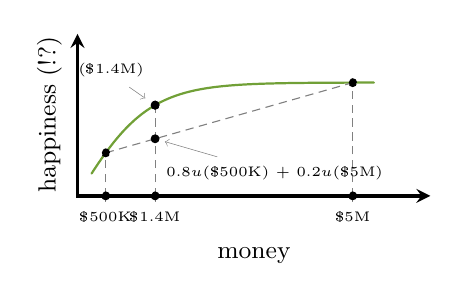
\begin{tikzpicture}
      \begin{axis}[
       width=0.5\textwidth,
       height=0.3\textwidth,
       axis line style={very thick, line cap=rect,},
       axis x line=bottom, axis y line=left,
       xmin=0, xmax=5, ymin=0, ymax=4,
       label style={font=\small},
       xlabel=money, ylabel=happiness (!?),
       xtick=\empty, ytick=\empty,
       extra x ticks={0.4,1.1,3.9},
       extra x tick labels={\$500K,\$1.4M,\$5M},
       extra x tick style ={font=\tiny},
      ]
      {\addplot [
       darkgreen, thick, line cap=round, smooth,
       domain=0.2:4.2, 
       samples=40
      ] {2.8*tanh(x)};}
      \addplot[mark=*,mark options={scale=0.7,black},densely dashed,gray] coordinates {(0.4,0) (0.4,1.063)};
      \addplot[mark=*,mark options={scale=0.7,black},densely dashed,gray] coordinates {(3.9,0) (3.9,2.797)};
      \addplot[mark=*,mark options={scale=0.7,black},densely dashed,gray] coordinates {(1.1,0) (1.1,2.241)};
      \only<3->{
       \addplot[mark=none,mark options={scale=0.7,black},densely dashed,gray] coordinates {(0.4,1.063) (3.9,2.797)};
       \addplot[only marks,mark options={scale=0.7,black}] coordinates {(1.1,1.41) (1.1,2.241)}
        node [pos=0,	pin={[pin edge={<-},pin distance=3pt]275:{\tiny 0.8$u($\$500K$)$ + 0.2$u($\$5M$)$}}] {}
        node [pos=1,	pin={[pin edge={<-},pin distance=3pt]95:{\tiny $u($\$1.4M$)$}}] {}
        ;
      }
     \end{axis}
     \end{tikzpicture}
    \end{center} 
    \item<2-> Based on this utility function, which one is more preferred?
    \begin{itemize}
     \item \$500K with probability 0.8, and \$5M with probability 0.2
     \item \$1.4M with probability 1
    \end{itemize}
   \end{itemize}
  \end{frame}
  
  \begin{frame}{Risk Attitudes}
   \begin{itemize}[<+->]
    \item Let $u$ be utility of an investor
    \item Lottery $A$ pays $\$x$ with probability $p$ and $\$y$ with probability $(1-p)$
    \item By utility theorem, $u(A) = pu(x) + (1-p)u(y)$
    \item Let $z  = \$(px + (1-p)y)$
    \item For a \alert<.>{risk-neutral} investor, $u(A) = u(z)$
    \item For a \alert<.>{risk-averse} investor, $u(A) < u(z)$
    \item For a \alert<.>{risk-seeking} investor, $u(A) > u(z)$
   \end{itemize}
  \end{frame}
  
  \begin{frame}{Are You a Risk-taker or Risk-seeker?}
   \begin{itemize}
    \setlength{\itemsep}{2em}
    \item<1-> Which one do you prefer?
    \begin{itemize}
     \item Lottery A: \$50 with prob 0.1 and \$0 otherwise
     \item Lottery B: \$5 with prob 1
    \end{itemize}
    \item<2-> How about these?
    \begin{itemize}
     \item Lottery A: \$5,000,000 with prob 0.1 and \$0 otherwise
     \item Lottery B: \$500,000 with prob 1
    \end{itemize}
   \end{itemize}
  \end{frame}
  
  \begin{frame}{Risk Attitudes (revisited)}
   \begin{columns}
    \begin{column}{0.7\textwidth}
     \begin{itemize}
      \item<1-> {\color{blue} Blue} has constant marginal utility $\longrightarrow$ risk-neutral
      \item<2-> {\color{darkgreen} Green} has decreasing marginal utility $\longrightarrow$ risk-averse
      \item<3-> {\color{red} Red} has increasing marginal utility $\longrightarrow$ risk-seeking
      \item<4-> {\color{gray} Gray} neither risk-averse nor risk-seeking
     \end{itemize}
    \end{column}
    \begin{column}{0.3\textwidth}
     \begin{center}
      \begin{tikzpicture}
      \begin{axis}[
       width=\textwidth, height=0.8\textwidth,
       axis line style={very thick, line cap=rect,},
       label style={font=\tiny},
       axis x line=bottom, axis y line=left,
       xmin=0, xmax=5, ymin=0, ymax=4,
       xlabel=money, ylabel=utility,
       xtick=\empty, ytick=\empty,
      ]
       \only<1->{\addplot [
        blue,thick, line cap=round, 
        domain=0:4
       ] {3*x/4};}
       \only<2->{\addplot [
        darkgreen, thick, line cap=round, smooth,
        domain=0:4, 
        samples=40
       ] {2.5*tanh(x)};}
       \only<3->{\addplot [
        red, thick, line cap=round, smooth,
        domain=0:3.6, 
        samples=40
       ] {5*(1+tanh(0.8*(x-4)))};}
       \only<4->{\addplot [
        gray, thick, line cap=round, smooth, 
        domain=0:4, 
        samples=40
       ] {1.25*(1+tanh(1.5*(x-1.7)))};}
      \end{axis}
      \end{tikzpicture}
     \end{center}
    \end{column}
   \end{columns}
  \end{frame}    
  
  \begin{frame}{Acknowledgment}
   \begin{itemize}
    \setlength{\itemsep}{1em}
    \item This lecture is a slightly modified version of ones prepared by
    \begin{itemizes}
     \item Asu Ozdaglar \href{https://ocw.mit.edu/courses/electrical-engineering-and-computer-science/6-254-game-theory-with-engineering-applications-spring-2010/index.htm}{[MIT 6.254]}
     \item Vincent Conitzer \href{https://courses.cs.duke.edu/spring16/compsci590.4/}{[Duke CPS 590.4]}
    \end{itemizes}
   \end{itemize}
  \end{frame}
 
\end{document}
